\documentclass{article}

\usepackage{amsmath, amsfonts, amsthm, amssymb}
\usepackage{fullpage}
\usepackage{textcomp}
\usepackage{graphicx}
\usepackage{subfig}
\usepackage{color}
\usepackage{verbatim}
\usepackage{float}
\usepackage{fancyhdr}
\usepackage{cancel}
\usepackage{lastpage}
\usepackage{cancel}
\usepackage{blindtext}
\pagestyle{fancy}
\renewcommand{\headrulewidth}{0pt}
\newcommand{\Mod}[1]{\ (\mathrm{mod}\ #1)}
\cfoot{\sc Page \thepage\ of \pageref{end}}

\newif\ifmarking
\markingfalse
\newif\ifsolutions
\solutionsfalse

\begin{document}
\noindent CSC384 A2 Written Answers\\
Zixing Gong\\
\begin{enumerate}
	\item Note that Pacman will have suicidal tendencies when playing in situations where death is imminent. Why do you think this is the case? Briefly explain in \textbf{one or two sentences}. (2 points total)\\
	Because if Pacman is about to die, then it would be better to die earlier rather than later score-wise.\\
	
	\item You should notice a speed-up compared to your MinimaxAgent. Consider a game tree constructed	for our Pacman game, where $b$ is the branching factor and where depth is greater than $d$. Say a	minimax agent (without alpha-beta pruning) has time to explore all game states up to and including	those at level $d$. At level $d$, this agent will return estimated minimax values from the evaluation function.\\~\\
	(a) In the best case scenario, to what depth would alpha-beta be able to search in the same amount of time? (1 point total)\\
	$O(b^{2d})$ (twice as deep).
	
	(b) In the worst case scenario, to what depth would alpha-beta be able to search in the same amount of time? How might this compare with the minimax agent without alpha-beta pruning? (2 points total)\\
	$O(b^d)$ if no pruning occurs, which is the same as normal minimax.\\
	
	\item \textbf{True or False}: Consider a game tree where the root node is a max agent, and we perform a minimax	search to terminals. Applying alpha-beta pruning to the same game tree may alter the minimax value of the root node. (1 point total)\\
	False, alpha-beta pruning will always give the minimax value for the root node as minimax would, however, if there are multiple optimal paths, we may get a different path with alpha-beta pruning.\\
	
	\item Consider a game tree where the root node is a max node, and the minimax value of the tree is $v_M$. Consider a similar tree where the root node is a max node, but each min node is replaced with a	chance node, where the expectimax value of the game tree is $v_E$. For each of the following, decide whether the statement is \textbf{True or False} and briefly explain in \textbf{one or two sentences} your answer.\\~\\
	(a) \textbf{True or False}: $v_M$ is always \textbf{less than or equal to} $v_E$. Explain your answer. (2 points)\\
	True, if we translate the minimax min node values into chance nodes, it would just have a probability of 1 for choosing the min child, with every other child being chosen with a probability of 0. Meanwhile a real chance node should never have probabilities of 0 or 1 (otherwise there is no chance involved), but even if it did, mathematically $v_M\le v_E$
	
	(b) \textbf{True or False}: If we apply the optimal \textbf{minimax} policy to the game tree with chance nodes, we are guaranteed to result in a payoff of at least $v_M$. Explain your answer. (2 points)\\
	False, consider the expectimax tree on the following page with probabilities on the right child flipped, so the new expected value is $19.83 = 0.99\times 20 + 0.01\times 3$. The $v_M$ value would be 5 (left child) in this tree, but minimax would choose the right child since the expected value of the right child is higher. But we could get unlucky and get a value of 3 from the right child instead of 20.
	
	(c) \textbf{True or False}: If we apply the optimal \textbf{minimax} policy to the game tree with chance nodes, we are guaranteed a payoff of at least vE. Explain your answer. (2 points)\\
	False, the expectimax value $v_E$ is an average of child values, so it is possible that by dumb luck the probabilistic opponent chooses a lower value than $v_E$.
	
	\begin{figure}[h]
		\centering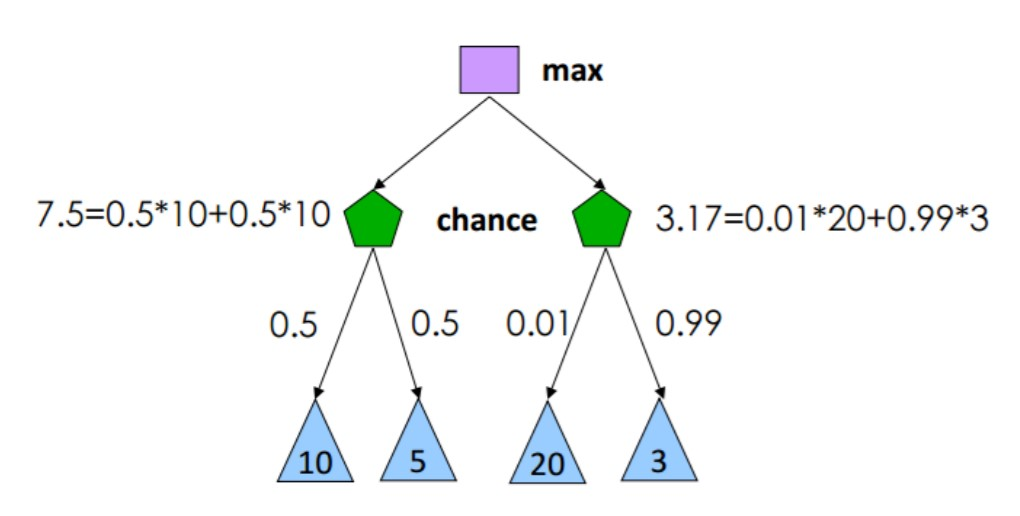
\includegraphics[width=\textwidth]{Expectimax.jpg}
	\end{figure}
\end{enumerate}\label{end}
\end{document}